\documentclass[tikz,14pt,fleqn]{article}

% Math
\usepackage[fleqn]{amsmath}
\usepackage{amssymb}
\usepackage{gensymb}
\usepackage{dsfont}
\usepackage{float}

% Insert dummy text
\usepackage{lipsum}  
% Allows to use caption*
\usepackage{caption}
% Scalable subfigures and subcaptions
\usepackage{subcaption} 
% Wrap text around figures
\usepackage{wrapfig}
% Code syntax highlighting
\usepackage{minted}
% Hyperlinks
\usepackage{hyperref}
% Customize page layout
\usepackage{geometry}
\geometry{a4paper, margin=1in}
% Page headers and footers
\usepackage{fancyhdr}
\pagestyle{fancy}
\fancyhf{}
\setlength{\parindent}{0pt}
\setlength{\parskip}{0.5\baselineskip}%

% includegraphics
\usepackage{graphicx}


\usepackage{cleveref}

\newcommand{\bmat}[1]{
   \ensuremath{
   \begin{bmatrix}
       #1
   \end{bmatrix}
}}
\newcommand{\pmat}[1]{
   \ensuremath{
   \begin{pmatrix}
       #1
   \end{pmatrix}
}}

\usepackage{hyperref}



\usepackage[utf8]{inputenc}


%%%%%%%%%%%%%%%%%%%%%%%%%%%%
%% VARIABLES
\newcommand\namesurname{Albert Cerfeda}
\newcommand\assignment{Assignment 2 - Image Classification}

\newcommand\subject{Machine Learning}
\newcommand\documentdate{1 June 2023}

% Title content
%%%%%%%%%%%%%%%%%%%%%%%%%%%%
\rhead{\assignment}
\lhead{\namesurname}
%%%%%%%%%%%%%%%%%%%%%%%%%%%%

\rfoot{Page \thepage}


\begin{document}

\begin{titlepage}
   \begin{center}
       \vspace*{0.2cm}

       \textbf{\Large{\subject}}

       \vspace{0.5cm}
        \textbf{\assignment}\\[5mm]
        
            
       \vspace{0.4cm}

        \namesurname
        \begin{figure}[H]
            \centering
        \end{figure}
       \tableofcontents

       \vspace*{\fill}
     
        
\includegraphics[width=0.4\textwidth]{fig/logo.png}
       
        \documentdate \\
        Università della Svizzera italiana\\
        Faculty of Informatics\\
        Switzerland\\

   \end{center}
\end{titlepage}


\section{Tasks}
In this assignment we are tasked in building neural networks with the goal of correctly classifying images from a dataset containing images of 7 different species of felines. The dataset is composed of 1697 samples and each image has $223\times 224$ resolution. The images are in color so they have 3 channels.

\subsection{Task 1}
In the first task we build a Fully Connected Feed Forward Neural Network (FFNN) for solving the classification problem.


\begin{figure}[h!]
\begin{subfigure}[t]{.49\linewidth}
  \centering
  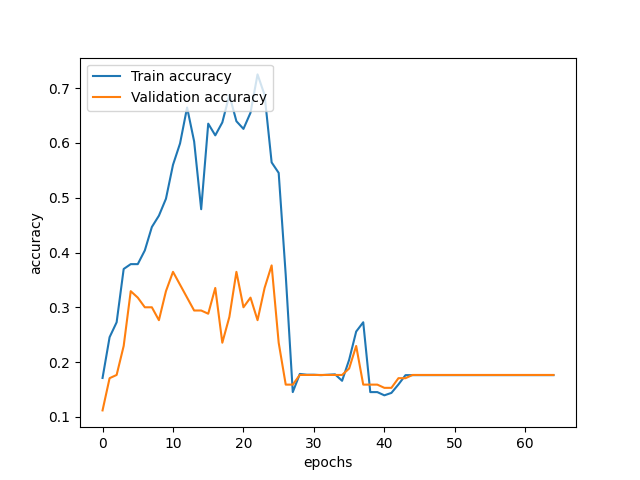
\includegraphics[width=\linewidth]{fig/out/T1.model_accuracy.png}
  \caption{Training accuracy and validation accuracy}
  \label{fig:t1.accuracies}
\end{subfigure}
\begin{subfigure}[t]{.49\linewidth}
    \centering
    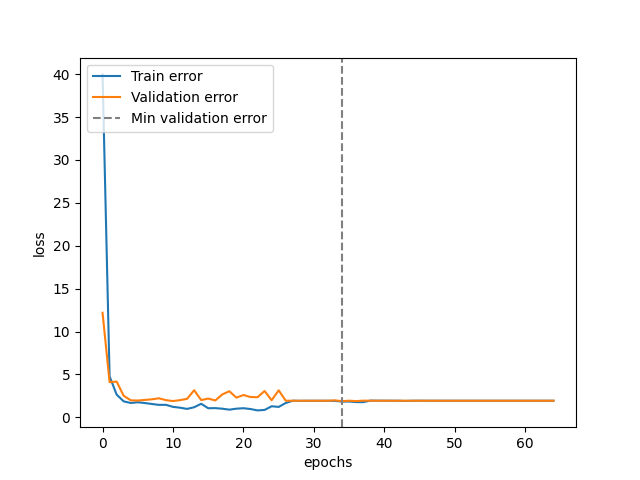
\includegraphics[width=\linewidth]{fig/out/T1.model_loss.png}
    \caption{Error rate}
    \label{fig:t1.losses}
\end{subfigure}
\caption{Basic T1 model metrics during training}
\label{fig:t1.metrics}
\end{figure}
\begin{figure}[h!]
\begin{subfigure}[t]{.49\linewidth}
  \centering
  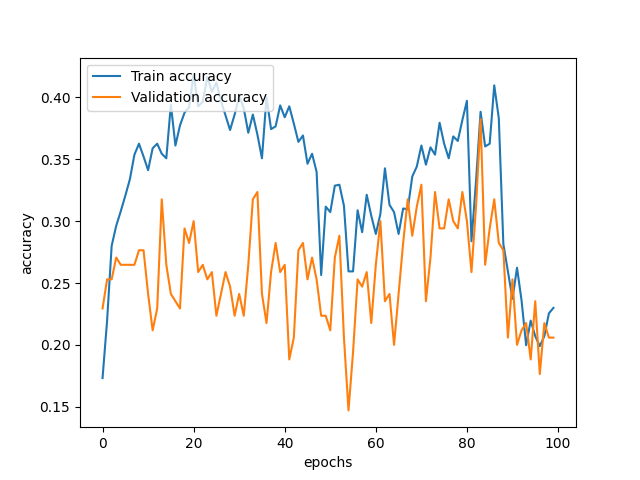
\includegraphics[width=\linewidth]{fig/out/T1-BONUS.model_accuracy.png}
  \caption{Training accuracy and validation accuracy}
  \vspace{-0.5cm}
  \label{fig:t1-BONUS.accuracies}
\end{subfigure}
\begin{subfigure}[t]{.49\linewidth}
    \centering
    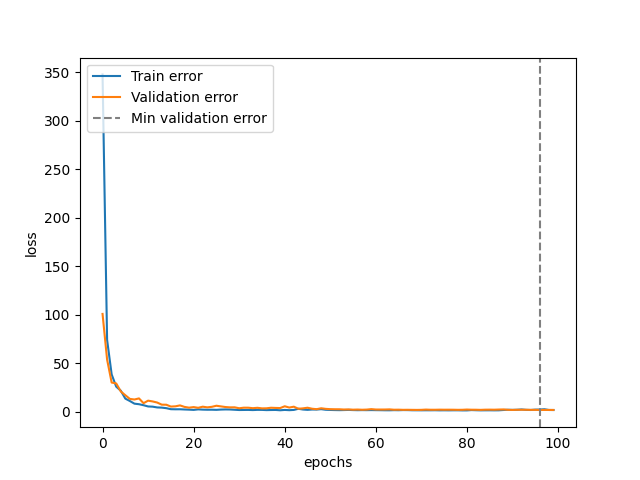
\includegraphics[width=\linewidth]{fig/out/T1-BONUS.model_loss.png}
    \caption{Error rate}
    \label{fig:t1-BONUS.losses}
\end{subfigure}
\caption{Bonus T1 model metrics during training}
\label{fig:t1-BONUS.metrics}
\end{figure}
We split the available dataset as such: $80\%$ train set, $10\%$ test set and $10\%$ test set.\\
We utilize the early stopping technique to avoid overfitting i.e we stop the training when the validation loss does not improve for a predefined amount of times.

\textbf{Basic T1 model}\\
Test Error: \textbf{1.86941}, Test Accuracy: \textbf{0.17647}\\
The basic T1 model respects the requirements of the exercise: no more than 3 layers, all layers are Dense, utilize the ReLu activation function for every neuron.

\textbf{T1 model for the bonus task}\\
Test Error: \textbf{2.04282}, Test Accuracy: \textbf{0.20000}\\
The T1 model for the bonus task is the same as the basic T1 model but with an additional Dense layer.

From our results we can see that our feed-forward neural networks are performing quite badly. This highlights the fact FCNNs are not very good at multi-class image classification for a number of reasons. The most important thing they are lacking is awareness of spatial continuity. Since every pixel is a separate feature, CNNs struggle a lot when trying to recognize patterns in image data. That is because the relative distance and spacing of the pixels is not taken into account. As a demonstration if were to evaluate the performance on the \textit{training set} we would get very good, biased results as expected, but were we to slightly so shift each image or perform any kind of manipulation on them, and we would see the error rise. Also in FCNNs since every layer is fully connected to the next, we have a very high number of parameters, rendering our model more computationally expensive and generally more prone to overfitting.

In our second model made for the bonus task, we do not have restrictions anymore on the input layer dimensionality of the FCNN. Instead of using the raw image pixel values as features, we have to perform some degree of feature extraction. We extract some features that can tell the neural network as much as possible on the nature of each image in the dataset, such as: mean and variance over the whole image, mean and variance for each channel, max and min values over the whole image, max and min values for each channel, ratios between statistics for each channel and image histograms.\\
Although we may are under the impression that we have richer, more descriptive data now, that is really not the case. By computing such metrics and not including the individual pixel values, we have more ambiguous data as every metric is computed by aggregating the image. In other words, images with the same mean or variance may not be the same image.\\
Our test results in fact show that our T1-BONUS model does not perform better. As a proof of what I stated above, I trained the same model on the pixel values \textit{plus} the extracted features, and the test error decreased significantly to about \textbf{1.5}. A possible approach to further improve the feature extraction would be to compute the fourier transform of each image. That is because most felines in the dataset have distinguishing traits based on their striped fur. Such alternating pattern on their fur would be noticeable in the fourier transform and therefore identifiable by the FCNN.


\subsection{Task 2}
 In this task we build a Convolutional Neural Network (CNN) for solving the classification problem. CNNs use convolutional layers which take into account the spatial structure of input images and learn local features, making them more effective at detecting patterns in images.\\
 \begin{figure}[h!]
    \begin{subfigure}[t]{.49\linewidth}
      \centering
      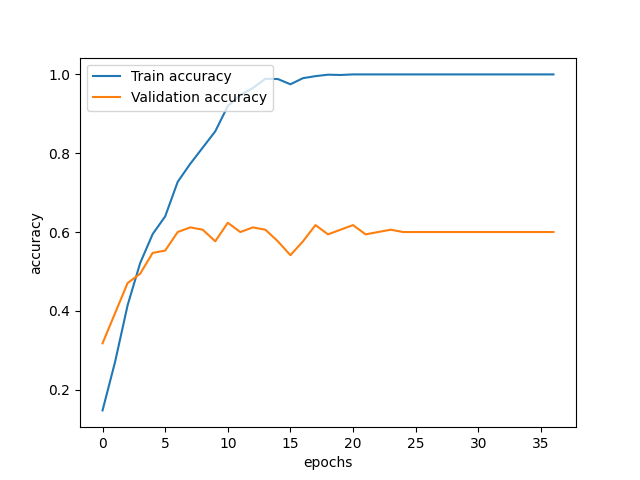
\includegraphics[width=\linewidth]{fig/out/T2.model_accuracy.png}
      \caption{Training accuracy and validation accuracy}
    \end{subfigure}
    \begin{subfigure}[t]{.49\linewidth}
        \centering
        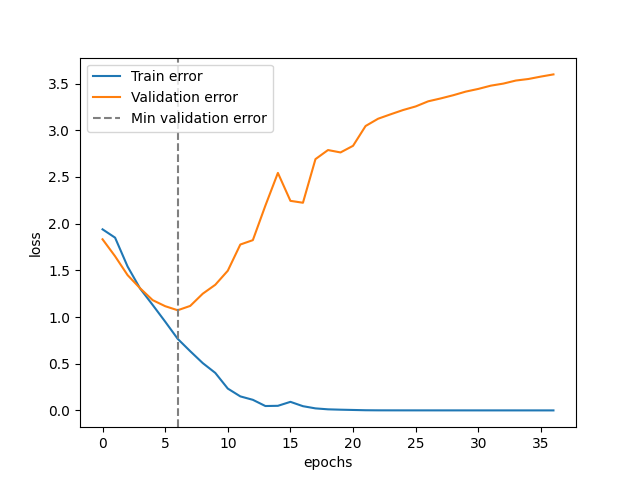
\includegraphics[width=\linewidth]{fig/out/T2.model_loss.png}
        \caption{Error rate}
    \end{subfigure}      
    \caption{The T2 model metrics during training}
    \label{fig:t2.metrics}
    \vspace{-0.5cm}
\end{figure}
\begin{figure}[h!]
    \begin{subfigure}[t]{.49\linewidth}
      \centering
      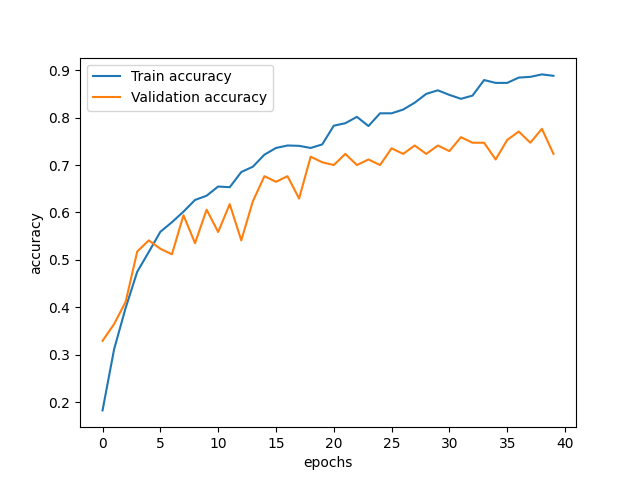
\includegraphics[width=\linewidth]{fig/out/T2.model_augmented_accuracy.png}
      \caption{Training accuracy and validation accuracy}
      \label{fig:t2-augmented.accuracy}
    \end{subfigure}
    \begin{subfigure}[t]{.49\linewidth}
        \centering
        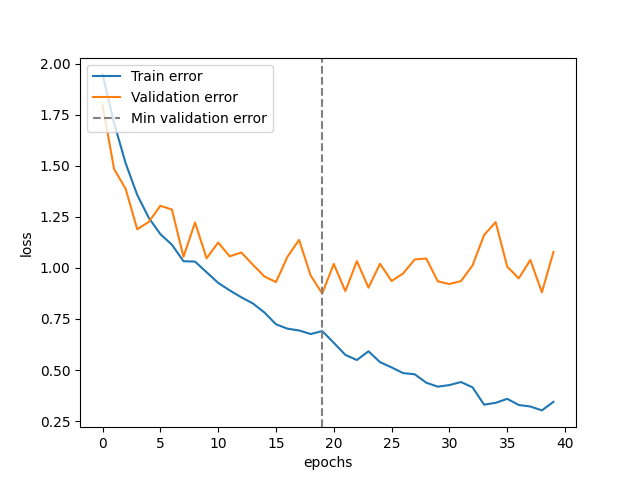
\includegraphics[width=\linewidth]{fig/out/T2.model_augmented_loss.png}
        \caption{Error rate}
    \end{subfigure}      
    \caption{\textit{Augmented} T2 model metrics during training}
    \label{fig:t2-augmented.metrics}
    \vspace{-0.5cm}
\end{figure}

The models respect the requirements of the exercise: utilize 3 convolutional layers, 3 pooling layers and 3 dense layers (output layer included).\\

\textbf{Basic T2 model}\\
Test Error: \textbf{0.93583}, Test Accuracy: \textbf{0.62353}

\textbf{\textit{Augmented} T2 model}\\
Test Error: \textbf{0.77835}, Test Accuracy: \textbf{0.74706}

\textbf{Bonus T2 model}\\
Test Error: \textbf{0.775862}, Test Accuracy: \textbf{0.741176}

When training with images, we have to take into account the variability of images. For example, our model has to be capable of classifying an image of a lion as such, independently from other image factors such as exposure, rotation, scale, saturation ecc. Even a slight change in the image can make it unrecognizable to our model. \autoref{fig:t2.metrics} shows the training and validation accuracy and error rate for the basic T2 model during training. In order to make our model more stable, we perform \textit{Data Augmentation}. That is, we augment our dataset by introducing many slight variations of our original image dataset. By expanding our dataset obtain a better model that yields better results. Notice how the model improves at a slower rate during training [\autoref{fig:t2-augmented.accuracy}]. It is possible that it is due to the fact that our dataset is more "diluted". Normally, the model would train on a much smaller and concise dataset with which the model learns quickly the main differences between the output classes. With the augmented dataset instead, the model will learn to thoroughly classify the data with better accuracy, but more extensive training is required for the model to train on every input class as the dataset is much larger now.

For the bonus task, we perform grid-search for finding the best hyperparameters to tune our model to.\\
When building the model, I defined two main hyperparameters that affect the structure and behaviour of the model: the \textit{learning rate} 
and the \textit{network downscale}. I introduced the network downscale hyperparameter for trying to reduce nedlessely large model sizes as much as possible while retaining the best prediction accuracy. For example a network downscale of 2 will halve the neurons for each layer by 2. I tried using \verb|GridSearchCV|, but deprecated modules plus other errors made me go for a simple for loop.

The grid parameters are the following: \textit{learning rate} can be chosen between 0.001, 0.0001 and 0.00005, while the \textit{network downscale} can be either 0.8, 1, 1.5, 2 or 3. Notice that a network downscale of 0.8 results in a network 20\% bigger.\\
After running the grid search, we obtain the best configuration of hyperparameters, i.e $$\text{Learning rate}: 0.0001, \text{Network downscale}: 2$$\\
By comparing the three models, we see how each of them is performing ever so slightly better, but not in a significative manner. The augmented model has better prediction capabilities than the basic model, but is extremely slow in training because of the augmented dataset. The Bonus model found through grid search is faster to the basic model, and also performs the best out of all the other models.

The models for trained for this assignment can be downloaded at the following link:\\
\href{https://drive.google.com/drive/folders/1eA\_jhffm-WtpzWtJAXAQplc8prVoZ708?usp=drive\_link}{https://drive.google.com/drive/folders/1eA\_jhffm-WtpzWtJAXAQplc8prVoZ708?usp=drive\_link}

\end{document}